\chapter{Introducción al Federated Learning}
\thispagestyle{fancy}
\fancyhead[LE]{\thechapter.Introducción al Federated Learning} 
Es de gran importancia comprender y conocer lo que es el Federated Learning para entender tanto el desarrollo, como la resolución de los problemas y retos que supone su implementación, por eso, en el presente apartado se explicará a conciencia de que se trata esta tecnología. 

\section{Información general}
El aprendizaje federado, es una técnica de aprendizaje automático que entrena un algoritmo a través de diversos dispositivos descentralizados, manteniendo siempre la información en cada uno de ellos (Fig\ref{fig:FedLearArquitectura}). El algoritmo que se busca entrenar en los dispositivos puede ser de cualquier tipo dentro del campo del aprendizaje automático, redes neuronales artificiales, aprendizaje profundo, árbol de decisión, etc. Por lo cual, se puede decir que el aprendizaje federado es una tecnología habilitadora para el entrenamiento de modelos de aprendizaje automático en redes de dispositivos.
\\ \\
Al contrario del aprendizaje automático convencional que reúne toda la información en un mismo computador, el aprendizaje federado busca entrenar un algoritmo en cada uno de los dispositivos que participen en la red, para luego combinarlos y conseguir un modelo de aprendizaje robusto. Los dispositivos que forman parte de esta red son denominados participantes y todos ellos forman la denominada como red de aprendizaje colaborativo. En esta red, todos aprenden de todos sin necesidad de compartir su información, consiguiendo mejorar la precisión y eficacia del algoritmo. 
\begin{figure}[thbp]
    \centering
    \fbox{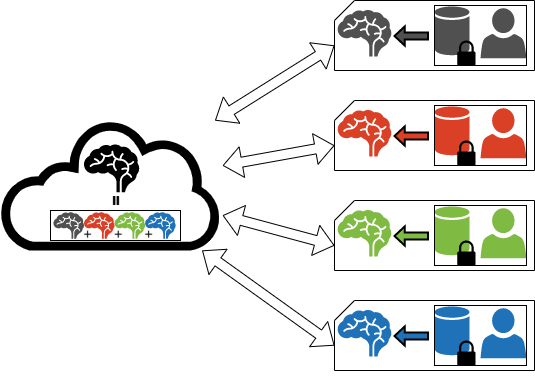
\includegraphics[width=0.5\textwidth]{Figuras/FedLeaConcept.png}}
    \caption{Diagrama de una red de Federated Learning} 
    \label{fig:FedLearArquitectura}
\end{figure}
\\ \\
Esta red permite repartir la carga de trabajo entre todos los participantes, puesto que cada uno se encarga de entrenar su propio modelo. Esto es posible gracias a que cada vez los dispositivos móviles tienen procesadores más rápidos y más potentes, lo que permite que sean capaces de realizar tareas más complejas y pesadas. De esta forma, se consigue que cada dispositivo sea propietario exclusivo de su información y no tenga que compartirla con ningún otro. Además, hoy en día los costes de comunicación son superiores a los de computación, por lo que cuanto más acciones se puedan computar en los dispositivos de los participantes menor será el consumo del entrenamiento del algoritmo. 
\\ \\
Sin embargo, debido a estas características propias del aprendizaje federado también sufre de grandes inconvenientes. El hecho de que la red está formada por diferentes participantes la hace heterogénea, con diferentes capacidades de cómputo y diferentes velocidades de conexión entre los distintos participantes, lo que puede incurrir en desconexiones o pérdidas de paquetes durante el proceso de aprendizaje.

\section{Fundamentos y Protocolo}
En general existen dos tipos de entidades en los sistemas de Federated Learning, los propietarios de la información (participantes de la red) y el propietario del modelo (servidor de Federated Learning). Los propietarios de la información entrenan localmente el modelo con la información de la que disponen, mientras que el propietario del modelo agrega los diferentes modelos recibidos de los participantes para mejorar el algoritmo. 
\\ \\
La comunicación puede ser llevada a cabo de diferentes maneras, de hecho, hay diseños de protocolos de aprendizaje federado como el desarrollado por los autores del trabajo \autocite{bonawitzFederatedLearningScale2019}, que lo dividen en 3 fases:

\begin{itemize}
    \item Selección de los participantes: El servidor elige un grupo de dispositivos conectados para participar en la red.
    \item Configuración: El servidor se configura en base al mecanismo de agregación definido y envía a los participantes el modelo global.
    \item Reporte: El servidor recibe la actualización de cada modelo de su respectivo participante. Más tarde los agrega usando el algoritmo elegido.
\end{itemize}

Además, estos autores definen un parámetro de población con el objetivo de limitar el acceso en caso de que haya muchos participantes, evitando que se conecten a la vez y saturen la red.

\section{Problemas presentes}
Como se ha mencionado antes, implementar el aprendizaje federado implica problemas y costes que hay que asumir y tratar con el objetivo de crear un sistema eficiente y estable. 
\\ \\
Cada actualización del modelo conlleva millones de parámetros, además se llevan tantas actualizaciones a cabo como precisión se quiera en el modelo. La gran dimensión de las actualizaciones puede incurrir en un aumento de los costes de conexión y generar un cuello de botella que puede verse agravado por los participantes, ya sea por la asimetría en las velocidades de internet o por la asimetría en la capacidad de cómputo. Es por eso, que para mejorar el rendimiento y reducir el coste de comunicación se deben considerar varias cosas.
\begin{itemize}
    \item En primer lugar, todos los dispositivos deben contar con una conexión estable, preferiblemente conexión por cable, o en su defecto conexión inalámbrica por Wi-Fi, descartando por completo todas aquellas conexiones por telefonía móvil.
    \item En segundo lugar, para minimizar el número de rondas de comunicación se puede realizar computación adicional en los dispositivos para que la agregación global se realice antes.
    \item También se puede reducir el tamaño de las comunicaciones, ya sea por compresión del modelo, compresión de los datos, o por el uso de una pequeña muestra representativa de estos en vez de enviarlos por completo.
    \item Por último, se pueden minimizar las actualizaciones de los modelos en base a la importancia de estas. Evitando enviar el modelo global hasta que este no suponga una clara mejora para los participantes.
\end{itemize}
